\chapter{Testing} 

SmartResolution is an open-source platform being marketed to those wanting to provide ODR services, and as such it is very important that the platform itself is thoroughly tested. Clients need to have confidence that the core platform works as it should, and module developers need to have confidence that the underlying system is robust enough to support their module. For these reasons, the core platform implementation was done alongside unit and integration tests throughout.

In an ideal world, the same principles would have been applied to the Maritime Collision module and to the SmartResolution website and marketplace. However, developing the core platform in a test-driven way turned out to be quite a slow, methodical process - read more in the evaluation section - and I felt that doing the same for the lesser two components was a luxury I could not afford with an impeding deadline. Therefore, this section is mostly concerned with testing the core SmartResolution software.

As previously mentioned, the project was developed in an agile way from mid-way through the design stage onwards. As such, the principles of business-driven development (BDD) and continuous integration (CI) were applied throughout the implementation. This section discusses the testing strategy that was applied during the implementation.

\section{BDD}

The project was developed in a business-driven way, as demonstrated in figure~\ref{uml:bdd}.

\begin{figure}[h!]
  \centering
    \ifimages
    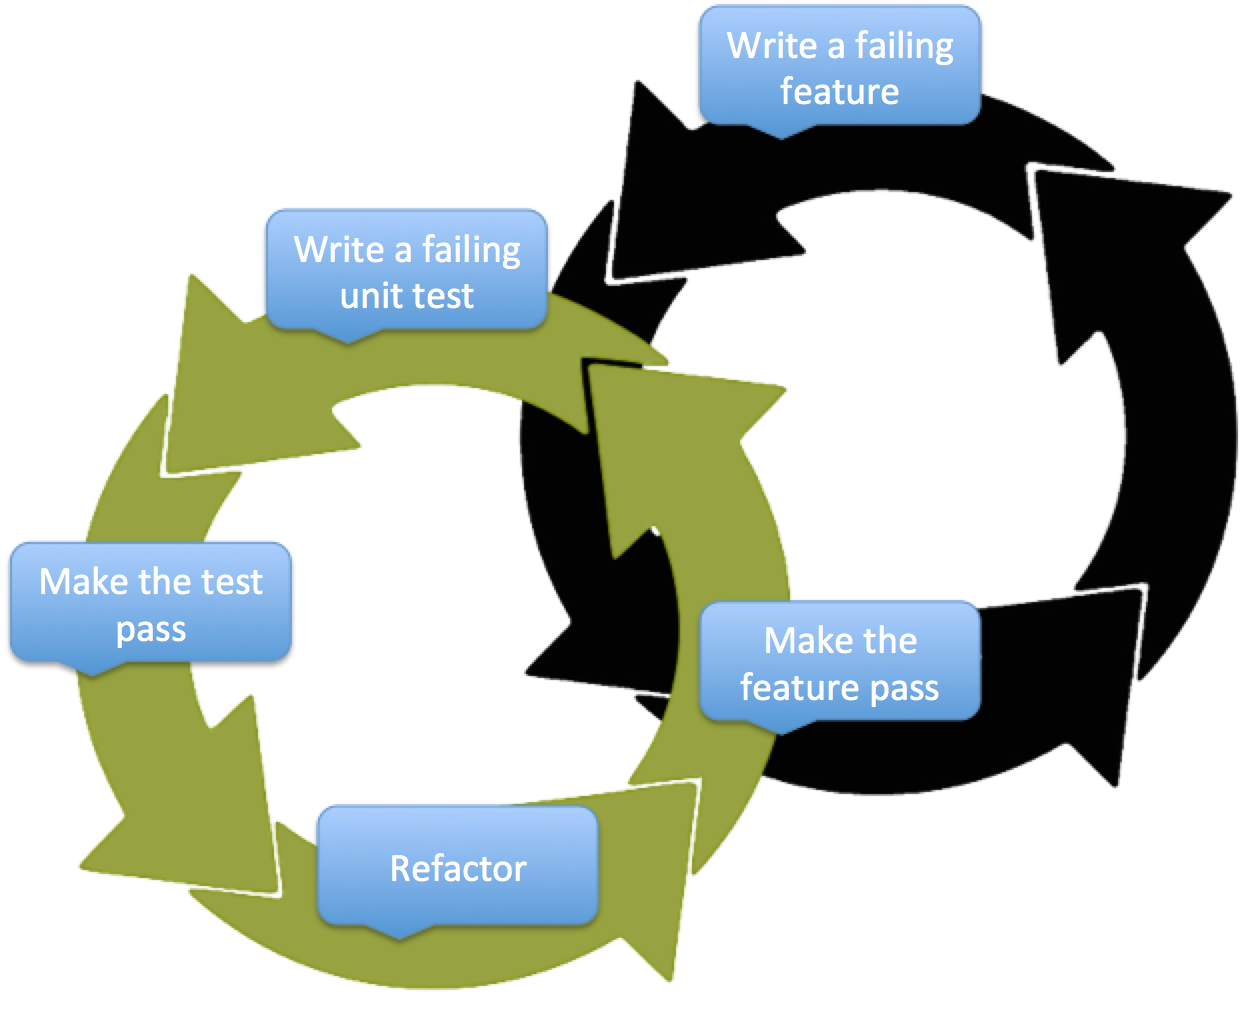
\includegraphics[width=\textwidth]{bdd}
    \fi
  \caption{The BDD development process: an extension of TDD}
  \label{uml:bdd}
\end{figure}

To begin with, a Cucumber feature is selected and executed. It should fail. Now a unit test is written to describe a low-level implementation of the feature. The unit test is run and again it should fail. The next step is to write the simplest code possible to make the unit test pass.

With the test passing, now is the opportunity to take a step back and look at the code in the context of the codebase as a whole. Can anything be refactored? If so, apply the refactoring step, then run the unit tests again to ensure that everything still works as correctly.

The unit-test process outlined above is known as the ``red, green, refactor" workflow and is repeated over and over until we have enough of the feature implemented to make a step of the feature pass, and then another step, and so on, until the feature as a whole is completed and passes the integration test.

Occasionally, features were too cumbersome to implement in a BDD manner, as they required spanning multiple architectures (routing, database layers, models, controllers, and so on). Wherever following BDD wasn't appropriate, I added unit and end-to-end tests post-implementation.

\section{Test database}

Cucumber regression tests are end-to-end and use a headless browser to emulate the browser environment, clicking buttons and filling in forms, then querying the state of the HTML to validate that an element of functionality worked as expected.

To accomplish this, the driver (in our case, Poltergeist) needs to be able to access the server. However, our tests rely on the database having certain fixture-data. Moreover, our tests will be making persistent changes to the database - so it's essential that the tests use a test database, rather than the production database.

As far as the server is concerned, Poltergeist sends a HTTP request, just like any genuine user on a normal browser. Poltergeist needed to be able to send a flag, to explicitly inform the application that the request is coming from a test suite and, thus, should be using a test database.

Poltergeist allows you to override the HTTP headers sent with each request, so my Cucumber tests modify the User-Agent property to be either \lstinline{Poltergeist} or \lstinline{Poltergeist--clear}. Both headers inform the application that it should use the test database, but the latter provides an additional instruction that the database should be cleared and re-populated with test data before processing the request. This is demonstrated in figure~\ref{uml:headers}.

The process of clearing the database involves removing the SQLite database entirely, creating a new SQLite database, executing the table-setup SQL (all performed via shell commands through PHP's \lstinline{shell_exec} function) and then seeding the database with fixture data. This fixture data is defined in \lstinline{data/fixtures/fixture_data.yml} and the mapping of YAML data to SQL tables is defined in \lstinline{data/fixtures/seed.php}.

\begin{figure}[h!]
  \centering
    \ifimages
    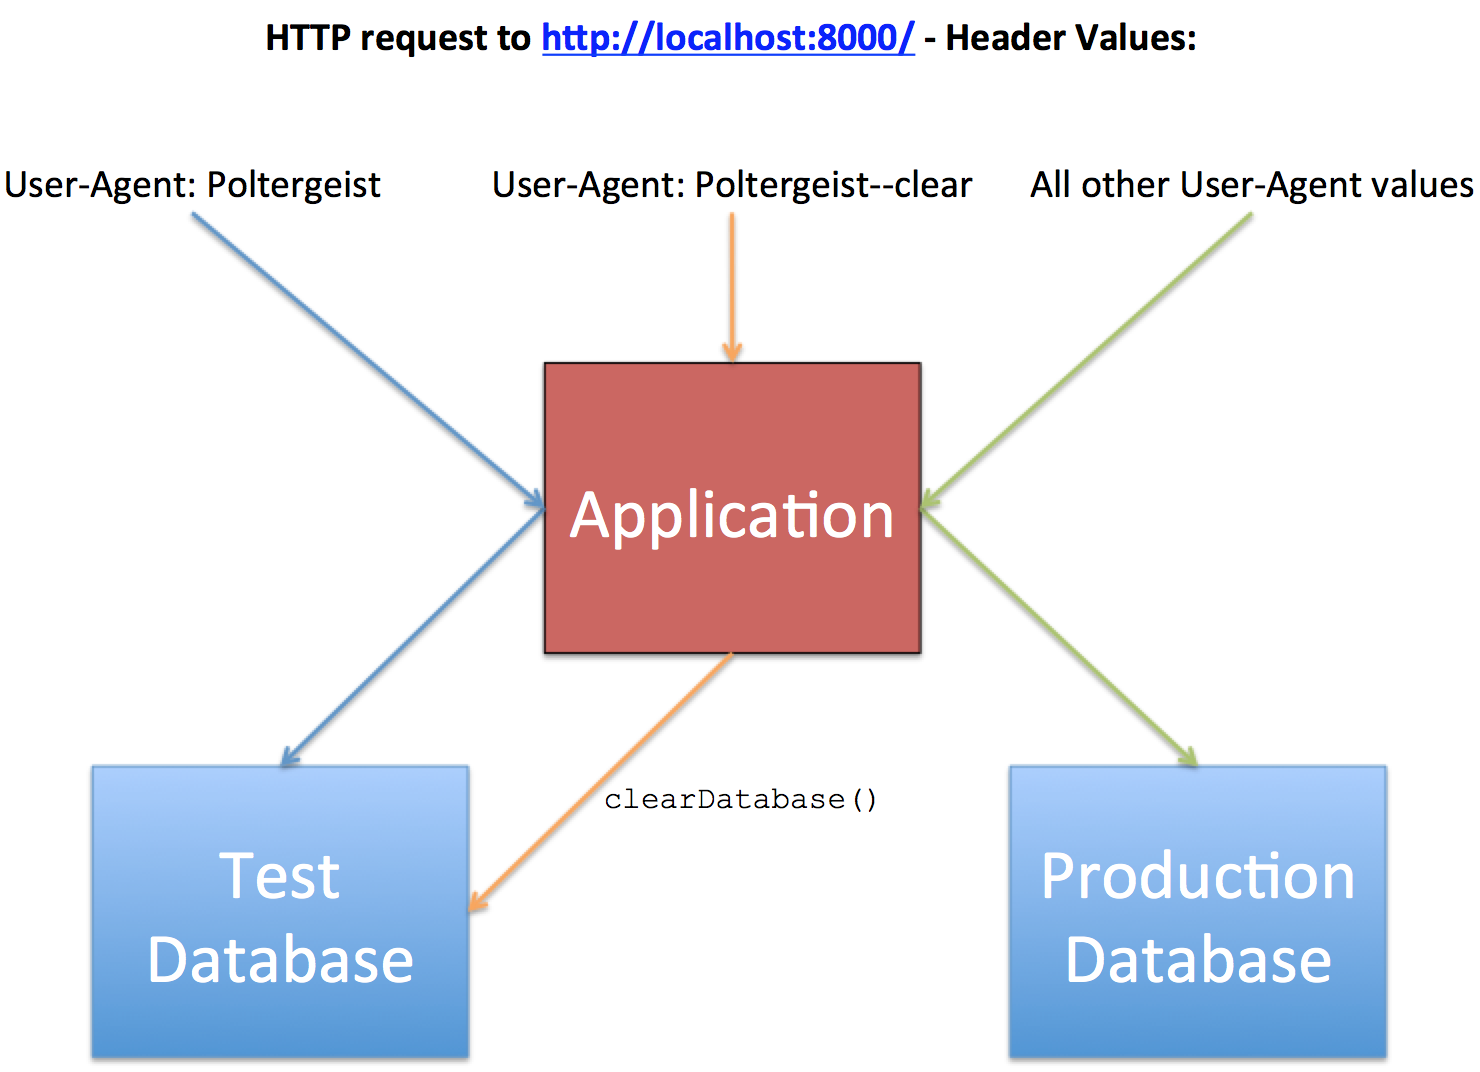
\includegraphics[width=\textwidth]{headers}
    \fi
  \caption{Visualisation of how SmartResolution determines which database to use depending on the received HTTP headers}
  \label{uml:headers}
\end{figure}

There's nothing stopping the end-user changing the headers that they send, so they too could access SmartResolution and interact with the test environment rather than the production environment. Ultimately, this is completely harmless. The test database is cleaned every time the test suite is run, so they would not even be able to sabotage the tests. This is a tried and tested technique, and has been adopted by companies including the BBC~\cite{bbc:cucumber}.

\section{Unit Testing}

Almost every class in the system has an associated unit test. This does not apply to library classes, such as those provided by F3, since the responsibility for testing those classes resides with the third party.

Unit tests verify that the publicly available methods of a class work as expected, both when accessed correctly and incorrectly. The nature of unit tests should be that they are loaded into memory and are very quick to run. ``Unit tests focus just on the class or method at hand. They run entirely in memory, which makes them very fast. Depending on your platform, your testing tool should be able to run at least 100 unit tests per second."~\cite{artOfAgile}

Some of the unit tests in SmartResolution are not `true' unit tests, as they rely on a database connection. According to Michael Feathers, ``A test is not a unit test if it talks to the database, it communicates across the network, it touches the file system or it can't run at the same time as any of your other unit tests.''~\cite{feathers:unitTests}

As with the Cucumber tests, some of my unit tests rely upon fixture data and, additionally, some unit tests might alter, add or remove items from the database, so the unit tests rely on and interact with the test database.

Generally speaking, it is more important to have a complete set of tests than a test suite that can be run quickly. That said, speed is important to the developer workflow, and was something that I concentrated on improving towards the end of the project.

\subsection{Database transaction threads}

\subsubsection{Database transactions and PHP}

Often, we want to accomplish several things in one `transaction', for example, debiting one person's account and crediting the other person's account. If the debiting of the first person's account fails - for example, if doing so would make their account balance negative - then we don't want the other person's account to be credited. Both queries must happen, or neither must happen.

Transactions are supported in PDO (PHP Data Objects) and in F3's wrapper for PDO, where we are able to define the start and end points of a transaction. The above example could be represented in code as follows, and if either query in the transaction fails, neither would be applied:

\begin{lstlisting}
$db->begin();
$acc1->debit(400);
$acc2->credit(400);
$db->commit();
\end{lstlisting}

\subsubsection{Issues with testing database transactions}

Between test suites, SmartResolution runs the `clear database' command to revert the test database to a known constant: an untainted database filled with predefined fixture data. This reverses any changes that may have been made to the database when running the previous test suite.

This is a useful technique in ensuring that test suites don't corrupt one another's results and that each suite works with the same set of data. However, it is slow and takes around a second on a reasonably powerful machine, becoming a problem if the script is called too often.

I made a conscious effort to keep these resets to a minimum, but a problem I faced early on in my unit tests was the following error message:

\begin{lstlisting}
PDOException: There is already an active transaction!
\end{lstlisting}

The exception refers to a situation in database transactions whereby a transaction was initiated, perhaps some queries were queued for the transaction, and then there was another request to begin a transaction. Somewhere in SmartResolution, a transaction was not being committed or rolled back.

This exception was usually raised after testing a part of my application that should (and does) raise an exception, such as trying to assign a law firm as the agent of a dispute. The expected exception was being raised and that was preventing the change (the assignment of the law firm to the dispute) from being made persistent, but subsequent attempts to begin new transactions complained that a transaction was already in progress.

Early on, this wasn't too much of an issue: I was able to run the `clear database' command between any unit tests that raised this exception, as removing and re-creating the database would naturally clear any outstanding transactions. This was a bit of a hack, but felt justified as the test and production environments are very different. In the test environment, hundreds of transactions are initiated when running the unit tests and all tests are hooking into the same database connection. In the production environment this would not happen: if an exception is raised, an error page is triggered and the user is faced with an error message relating to the exception. Once PHP delivers the error page to the user's browser, the database connection is no longer open and thus a new transaction can begin.

For several weeks, I was happy with this solution, but it did mean that my tests were quite slow to run. You can see in a Travis build around that time that it took almost a minute to run 90 unit tests\footnote{A build on 15th April, before refactor: \url{https://travis-ci.org/ChrisBAshton/smartresolution/builds/58603809}}, violating James Shore's principle that unit tests should run almost instantly.

Eventually, I decided to spend some time investigating the issue. I deduced that the transaction was not being committed because an exception was being raised before it could be committed. What I did not realise was that transactions were not being automatically rolled back when an exception was raised - it was something that needed to be handled manually in each exception.

Handling the transaction rollback in each raised exception would mean writing code like this:

\begin{minipage}{\textwidth}
\begin{lstlisting}
$db->begin();

// several lines of code and database queries

if (// some condition) {
    $db->rollback();
    throw new Exception('Error!');
}

// more lines of code and database queries

if (// another condition) {
    $db->rollback();
    throw new Exception('Another error!');
}

$db->commit();
\end{lstlisting}
\end{minipage}

This seemed laborious, error-prone and messy. Instead, I defined a custom exception function which throws an exception, but also rolls back any existing transactions.

\begin{minipage}{\textwidth}
\begin{lstlisting}
    public function throwException($message) {
        try {
            Database::instance()->rollback();
        } catch (Exception $PDOException) {
            // do nothing - we only wanted to roll back the transaction if one existed.
            // since one doesn't exist, there's nothing to roll back. Let's just continue and
            // throw the Exception we wanted to throw in the first place.
        }
        throw new Exception($message);
    }
\end{lstlisting}
\end{minipage}

Now that the root of the problem had been fixed, unit tests could be run without clearing the database in between each test. This led to big improvements in test speed: at this stage, I could now run 112 unit tests in 34 seconds.\footnote{A build on 17th April, after refactor: \url{https://travis-ci.org/ChrisBAshton/smartresolution/builds/58932345}} This is 3.29 unit tests per second (UTPS), compared with 1.58 UTPS before the optimisation.

I still needed to clear the database between each test \emph{suite}, as the tests would still alter the state of the database. But now, by and large, most of the tests \emph{within} those suites did not need to run on a new database connection.

\subsection{Refactoring to pure unit tests}

Earlier I described how `pure' unit tests should not query a database. An unfortunate consequence of the implementation of my code was that database querying was essential to unit test my classes, as my models were populated by an ID representing a row in the database, rather than populated with an array of data which may or may not have come from a database.

For example, the \lstinline{Message} class expected to be passed an ID to its constructor. Inside the constructor, a function call was made to a data wrapper class which contained the business logic for retrieving from the database the class-specific data (such as message content, author ID, etc) corresponding to the given ID. The returned array was then used to populate the model. This somewhat decoupled the model from the database - all SQL queries were encapsulated in the intermediary database querying objects - however, it made the models quite difficult and slow to test.

The decision to implement the models like this was to make life easier for the controllers. Let us examine this with some pseudo-code:

\begin{lstlisting}
// inside a controller
$disputeID = getDisputeIDFromUrl();
$dispute = new Dispute($disputeID);
\end{lstlisting}

Inside the Dispute model, we had something like this:

\begin{minipage}{\textwidth}
\begin{lstlisting}
function __construct($disputeID) {
    $disputeDetails = DisputeDatabaseConnector::getDisputeDetails($disputeID);
    $this->title = $disputeDetails['title'];
    // and so on
}
\end{lstlisting}
\end{minipage}

Though the model was made a little impure due to the database connection object, I could write nice code in the controllers that only had to worry about getting an object's ID. This meant that I could chain method calls together, passing returned IDs into subsequent constructors to quickly and easily get the objects I needed.

\subsubsection{Refactored solution}

Refactoring constructors to take arrays of data rather than IDs took some significant effort and meant extracting the database querying out of the models:

\begin{lstlisting}
// inside the Dispute model
function __construct($disputeDetails) {
    $this->title = $disputeDetails['title'];
    // and so on
}
\end{lstlisting}

The database query instead had to be moved to the controller;

\begin{lstlisting}
$disputeID = getDisputeIDFromUrl();
$disputeDetails = DisputeDatabaseConnector::getDisputeDetails($disputeID);
$dispute = new Dispute($disputeDetails);
\end{lstlisting}

The advantage of the refactored solution is that the models become pure: they now have no concept of a persistence layer. We can now test our models by passing arrays of hard-coded data, removing the need to retrieve from and write to a database.

Changing object constructors to take arrays rather than database record IDs meant I could cut down test times significantly. After implementing the refactored solution, my test suite performed 109 unit tests in just 12.7 seconds: a UTPS of 8.57.\footnote{A build on 22nd April, after final refactor: \url{https://travis-ci.org/ChrisBAshton/smartresolution/builds/59532839}} This information is summarised in comparison table~\ref{table:testTimes}. It is worth noting that those are the results on Travis: on my MacBook Pro, the entire unit test suite runs in under six seconds.

\begin{table}[h!]
\label{table:testTimes} 
\begin{center}
\begin{tabular}{ l | r | r | r | r | r}
  Stage in project & Unit tests & Assertions & Time taken (s) & UTPS & APS \\
  \hline
  Pre-refactor & 90 & 221 & 57.70 & 1.58 & 3.83\\
  Fixed database transactions & 112 & 263 & 34.24 & 3.29 & 7.68\\
  Refactored to use only pure models & 109 & 309 & 12.72 & 8.57 & 24.29
\end{tabular}
\end{center}
\caption {Table showing the unit test times after various refactoring steps}
\end{table}

\subsubsection{Further refactoring}

Extracting the database retrieval out of the model also meant extracting the database \emph{changes} out of the model. I took the opportunity to refactor this behaviour too.

Beforehand, I had code like this inside my models:

\begin{lstlisting}
// inside the Dispute model
function closeSuccessfully) {
    SomeDatabaseConnector::updateField('disputes', 'status', 'resolved', $this->disputeID);
}
\end{lstlisting}

This was tightly coupled to the underlying table representation, and became fiddly when having multiple functions that change different fields. When moving this behaviour into the controllers, I decided to encapsulate all updates inside one update method that corresponds to the model:

\begin{lstlisting}
// inside the Dispute controller
$dispute->closeSuccessfully();
$update->dispute($dispute);
\end{lstlisting}

Instead of updating an individual field value, I now pass the entire Dispute object to an update method which knows how to map the dispute object to its representation in the database. It calls the necessary methods on the dispute object (such as \lstinline{$dispute->getStatus()}) to collect all of the information it requires to update the record. 

This large refactoring task perhaps hints at a broader problem: object-relational mapping. It could be argued that at various points in my codebase I have not approached the problem in the object-oriented way I should have, because I've had to manually map the object to be in terms of its underlying relational database representation. Perhaps, in hindsight, an object-relational database would have been more appropriate than an RDBMS, to delegate the understanding of the object-relational mapping to a third-party.

\section{Functional Testing}

Every feature of the SmartResolution core software is defined as a Cucumber feature, associated with step definitions, to make each feature executable and automatically verify that the system is working as expected. As a reminder, the full list of tested features is outlined in appendix~\ref{appendix:requirements}, and the justification for the choice of Ruby and Cucumber as the BDD framework is in appendix~\ref{appendix:bdd}.

Unit tests are tightly coupled to the specific implementation of the code, making refactoring difficult if you wish to move methods, rename classes and the like. A necessary principle of unit tests is that the tests will break if the code changes its external API. These tests are highly valuable but do not offer complete code coverage, since there are no tests to verify that the classes the unit tests are testing are even being used by the core system at all!

Cucumber features test the expected end-to-end functionality of the system as a whole and can be defined completely separately from the software itself. They are slower to run, but fill me with more confidence than unit tests, since they test the behaviour of the application from the point of view of the user, not the compiler.

\subsection{Functional tests structure}

Every Cucumber feature has a corresponding step definition. It's worth noting that, though it is not required to give the step definition file the same name as the corresponding feature file, this is the Cucumber convention and is regarded as best practice.

A Ruby step definition defines a step in a Cucumber scenario in terms of interacting with the page, through methods provided by the Capybara acceptance test framework. Capybara requires a browser driver such as Poltergeist to request and then render the webpage. The browser can be headless (running as a background process, hidden from view) or a window browser. Poltergeist, as the name might suggest, is headless.

As I began filling out my step definitions, I found that more and more steps were relying on methods and variables defined in other step definition files. In cases such as this, it was clear that a common helper class should be created. For example, step definitions have access to a `Session' helper class which provides methods to log in with specific credentials, or log into account types (e.g. \lstinline{Session.login_as_agent}). Figure~\ref{uml:cucumber} demonstrates the relationship between a Cucumber feature, its step definition, and the helper classes.

\begin{figure}[h!]
  \centering
    \ifimages
    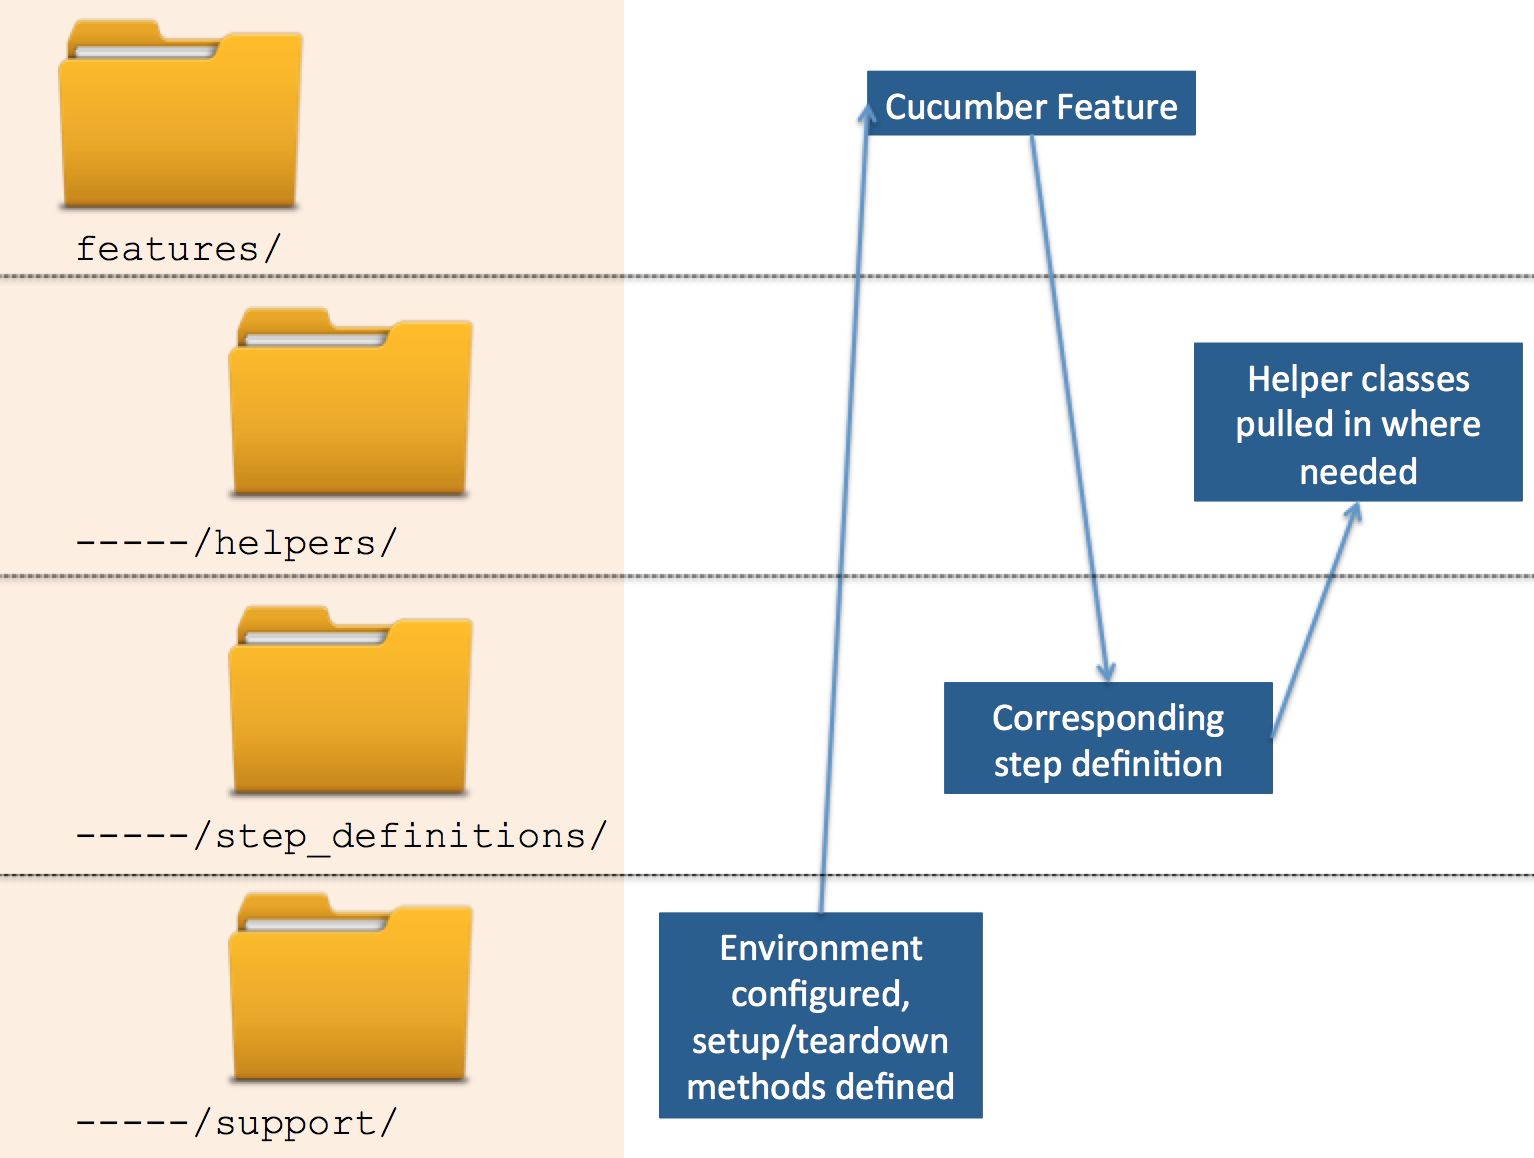
\includegraphics[width=\textwidth]{cucumber}
    \fi
  \caption{Visualisation of which files are involved in defining a Cucumber feature}
  \label{uml:cucumber}
\end{figure}

Finally, there are also numerous steps which are repeated across different features, such as ``Given I am logged into an Agent account". In cases such as these, it became difficult to maintain those step definitions when it could have been buried in any of the step definition files whose features depend on it, so these were extracted to a `\_common.rb' step definition file. This is now the first place one should look when trying to find and maintain a step definition.

\subsection{A note on feature style}

There is a trade-off between having a verbose Cucumber feature and a verbose step-definition. The former bogs the feature down in detail and risks devaluing it, whereas the latter can make maintenance more difficult.

I argued this same internal battle in the \emph{Developing Internet-Based Applications} assignment, discussing the pros and cons of each in some detail. The relevant extract of that report is included here in appendix~\ref{appendix:cucumber}.

My conclusion was that, though the two need to be balanced, it isn't detrimental to specify specific fields and error messages in the Cucumber feature itself. The alternative - abstracting that information away in the step definition - can make it difficult to maintain state throughout the scenario. Following this conclusion, some of the Cucumber features decided upon in the initial requirements were later reworded to fit in with this philosophy, though their purpose and relevance remained the same.

For example, this was an original `lifespan negotiation' scenario:

\begin{lstlisting}
  Scenario: Accepting a Dispute lifespan offer
    Given the other Agent has sent me a Dispute lifespan offer
    Then I should be able to accept the offer
    And the Dispute should start
\end{lstlisting}

This is how the scenario looks now that the step definitions have been implemented:

\begin{lstlisting}
  Scenario: Accepting a Dispute lifespan offer
    Given the other Agent has sent me a Dispute lifespan offer
    Then I should be able to Accept the offer
    And I should see the message 'Dispute starts in'
\end{lstlisting}

The original and amended scenarios are very similar, but the latter is a little more tied to the implementation. The `I should see the message' step definition is reused across many scenarios and means that the step definitions as a whole are simpler and cleaner, even if the Cucumber features themselves are slightly more verbose than before.

\section{Continuous Integration}

Travis CI ran all unit and functional tests on every pushed commit or pull request, automatically notifying via email if anything broke. It was an invaluable tool throughout the project and was well worth spending time configuring.

The most difficult aspect to setting up Travis was getting the PHP server running, since Travis only supports one terminal window. The PHP server had to be set up as a background process so that Travis could continue to run the other commands required to run the tests.

Travis wasn't the only tool that performed a service on every pushed commit. Just as important as ensuring that all tests continue to pass is ensuring that dependencies remain up-to-date. Gemnasium periodically checks the status of SmartResolution's dependencies and warns via the embedded SVG in the project README whether or not a newer version is available.

Dependency tracking is important, as newer versions of dependencies fix bugs and vulnerabilities discovered in older versions. By not updating SmartResolution's dependencies regularly I would risk crackers being able to exploit unpatched vulnerabilities. This is especially relevant since SmartResolution is open-source and anybody can see which version of which third-party library SmartResolution is using.

Another important thing to monitor with each commit is code quality, something that CodeClimate is trying to automate. Whenever I push a commit to SmartResolution, CodeClimate queues another scan of the codebase and informs me on a level of 1-4 whether the quality of my codebase has improved or deteriorated, using metrics such as variable name length, code duplication, the number of possible paths through a block of code, and so on. Utilising this third-party service helped fight the temptation to hack a bit of functionality in, instead encouraging good engineering practice and providing suggestions as to how the codebase could be made more maintainable.

\section{User Testing}

Whereas it is the software engineer's responsibility to ensure that the project is built right, it is the client's responsibility to ensure that the right project is built. Therefore, user testing with the client is critical.

As has already been highlighted, the customer for this project was extremely busy and was unable to meet more than a couple of times. This made user-testing very difficult, but I tried my best to offer alternative options.

It was good that I spent so long clarifying requirements at the beginning of the project. In the absence of regular communication and feedback, this original set of features was invaluable in ensuring that the system contained all of the required functionality.

Mid-way through the project, I deployed SmartResolution to smartresolution.org and invited all stakeholders to try out a beta version of the project, describing how to log into the system, what functionality had already been implemented, and what functionality had yet to be implemented.

Throughout development I adhered to the agile principle of regular releases, pushing the latest stable version of SmartResolution to the website on a daily basis so that the customer would be able to feel the benefit and experience a more feature-complete demo.

Later on in the project I made it even easier to demo the software, by producing a short video demonstrating the software and the maritime collision module. This is embedded on the homepage of smartresolution.org and enables users to see what the system is capable of without having to manually log in and out of demo accounts representing different user roles.

Where feedback was lacking from the customer, I turned to friends, family and the Twitter community to try out the demo and give me constructive comments to work on. These comments were fed back directly into my design, leading to the following improvements:

\begin{itemize}
\item Smaller icons. My early designs used dashboard icons around 3 times larger than the final design. I was trying to emulate clear and minimalist dashboards such as the one on DigitalOcean (see figure~\ref{screenshot:digitalOcean}) but my implementation was something consistently questioned in the feedback I received.
\item Larger font size. Bootstrap's default font was too small given the sparseness of the design as a whole. I increased the base font size; all font sizes across the site increased in size proportionally, as my CSS defined fonts in terms of \lstinline{em}.
\item Responsive improvements. It was never a requirement to make the SmartResolution software fully responsive: the fact that Bootstrap supports responsiveness by default was just an added bonus. However, some of my design decisions - such as absolutely positioning the lifespan status at the right hand side of the dispute - made for a poor experience on mobile. When this was pointed out in the feedback, I added a media query so that the positioning would only apply on devices of a minimum screen width.
\end{itemize}

\begin{figure}[h!]
  \centering
    \ifimages
    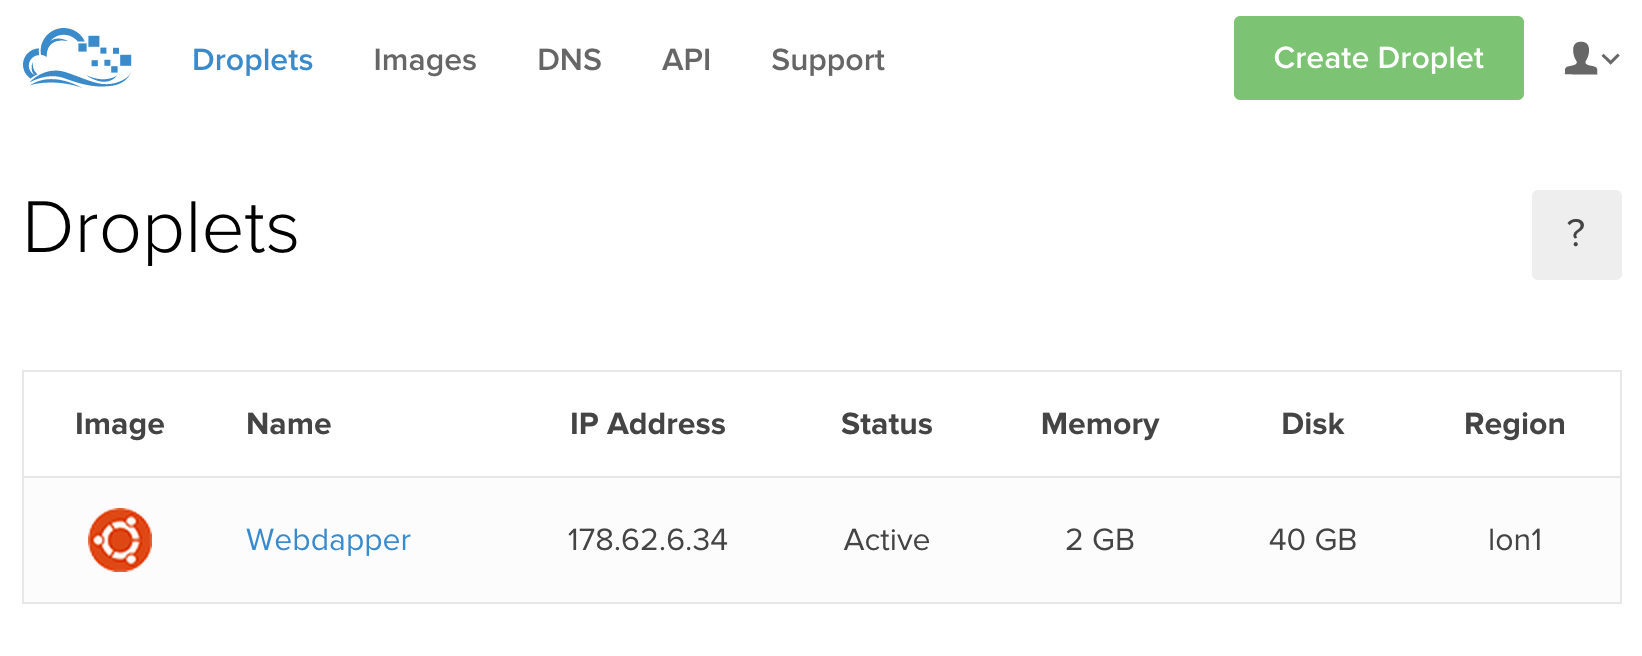
\includegraphics[width=\textwidth]{digitalocean}
    \fi
  \caption{Screenshot of the clean and simple DigitalOcean interface I wanted to emulate in the design for SmartResolution}
  \label{screenshot:digitalOcean}
\end{figure}

Feedback regarding the workflow of a dispute had to be treated differently, since the customer was the law expert and the people giving feedback were not law experts. However, their comments were collected and fed back to the law expert for trying to negotiate simpler dispute workflows.

One of the original requirements was for a formal resolution-offering process. An agent would be able to make an offer by filling in a HTML form denoting offer details, damages awarded, and so on. I was able to simplify this in light of the feedback: agents are human beings and can reach that kind of resolution through the communication option alone. They can then close the dispute successfully, with no need to officially form a structured offer that SmartResolution understands. Removing these artificial constraints made for a more user-friendly workflow and reduced the development overheads significantly.